\section{Motivating example}
%-------------------------------------------------------------------------------
The crux of the trace forensics problem is: How can we provide hints of proximal causes when an execution fails?

\begin{figure}[h]
\center{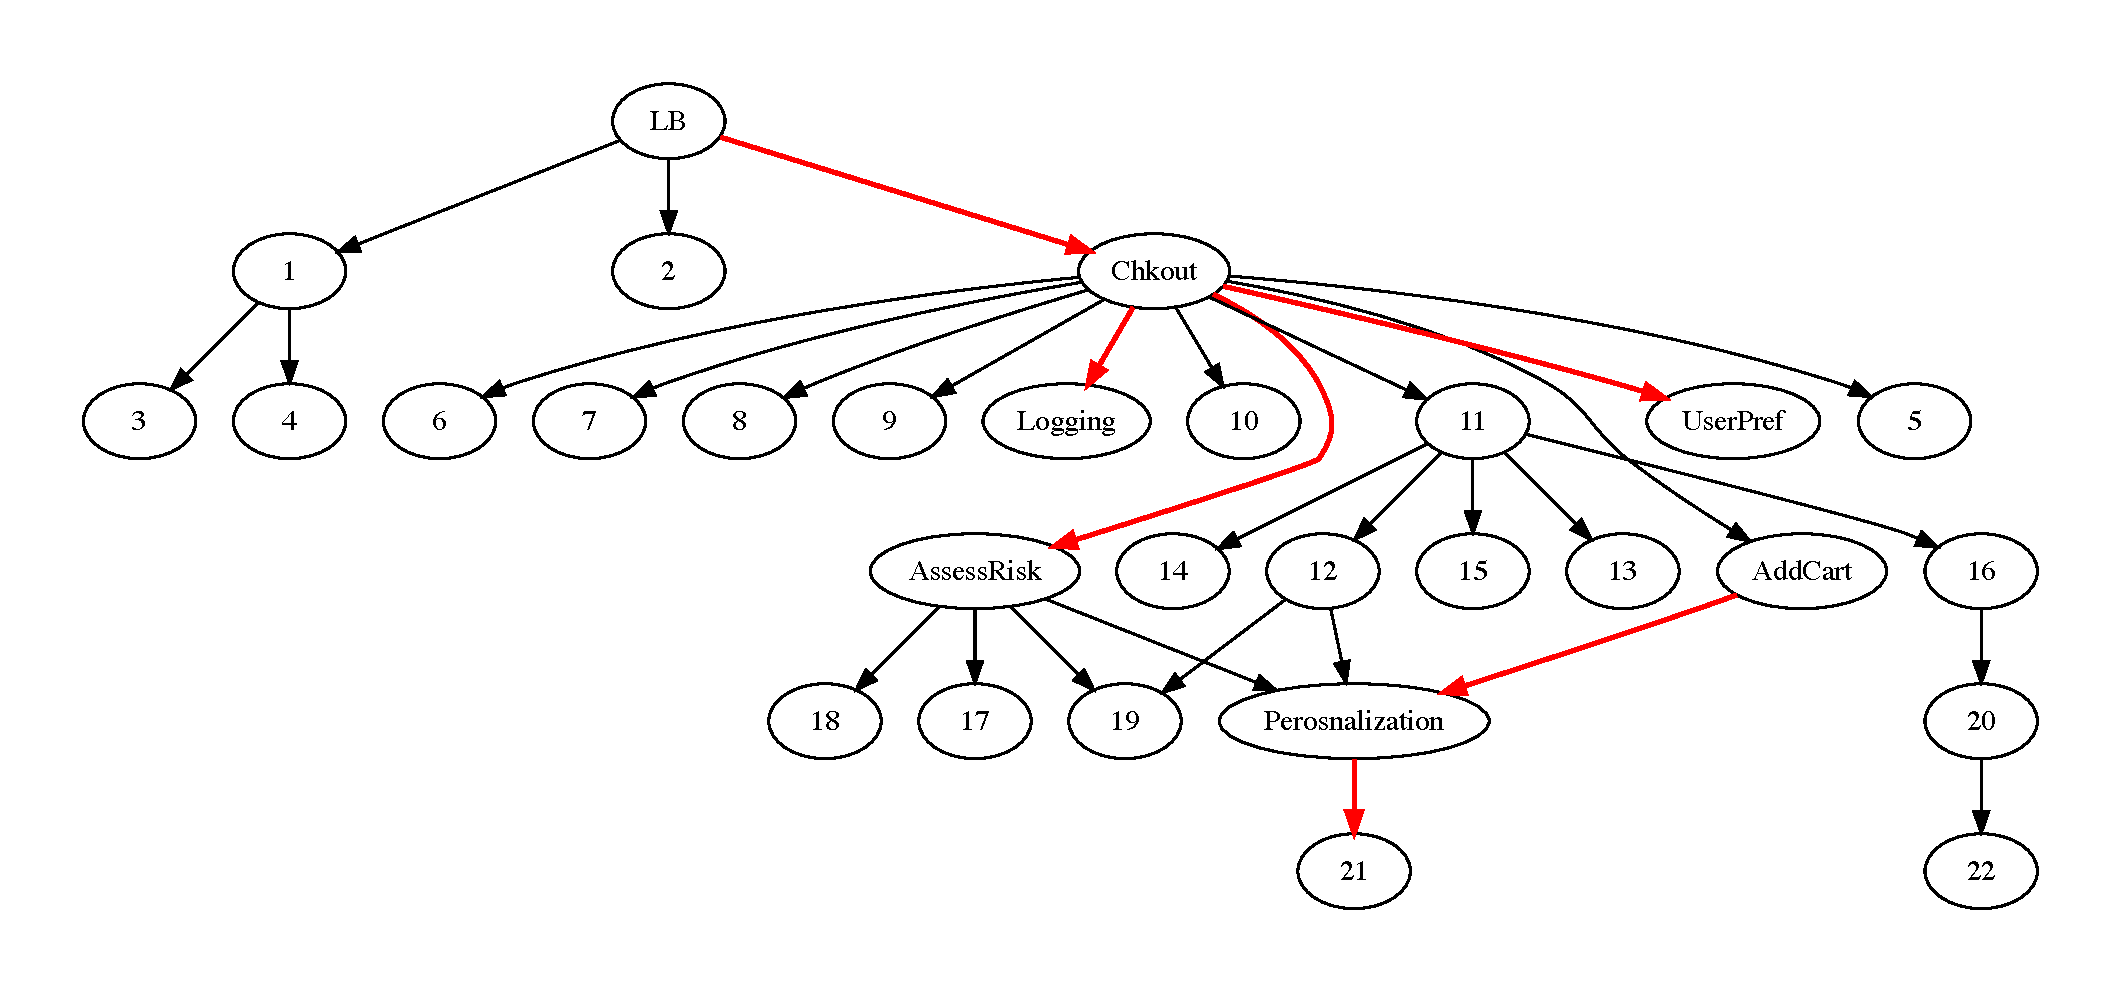
\includegraphics[scale=0.25]{anon_adrbk_fail.pdf}}
\caption{Example graph drawn from trace of a failed interaction. The red lines indicate that the callee has returned an error message to the caller}
\label{Failed_ex}
\end{figure}

Figure~\ref{Failed_ex} shows the  call-graph of a user interaction involving checkout of items for a cart, which ultimately fails. A successful checkout occurs when the user is able to place an order, else the checkout fails. When failures are observed, it is the job of a site reliability engineer (SRE) to troubleshoot the failure. Currently, the SRE sees a number of alerts from the monitoring system that maintains aggregate data over sliding windows of time for all services. The SRE might go about their job like so:
\begin{itemize}
\item Figure out which of the alerts are smokescreens to be ignored. \newline
Some services that are called as part of the interaction which provide useful functionality, but the failure of which can be tolerated by the system. These can be thought of as nice-to-have services. Alerts from such services may be safely ignored and an SRE would generally be able to identify these with experience.
\item Use domain knowledge about the dependencies between services to know which alerts are the result of transitive dependencies and must be ignored. \newline
As an example, the load balancer (LB) in the figure will be alerting. An intelligent SRE would conclude that since checkout (Chkout) has multiple downstream alerts, the alerts at LB are probably a result of the error being propagated up and try to dig deeper into one of the downstream alerts that look promising. Once a promising alert has been found, it is now time to look at the logs from the appropriate time to try to determine cause of failure.
\item Determine if the absence of some service(s) caused the failure \newline
Failures are sometimes caused by failure of mandatory services or a fallback path not being taken. Details of a network connection failure or time out in attempting to connect to downstream services might be buried deep in the logs, taking longer to unearth and fix, resulting in larger user downtimes. 
\end{itemize}


In the next section, we describe the generation of trace embeddings and the corresponding distance measure used. In the evaluation, we describe how we use the fairly simple operations on the embeddings to address the problem described above and automatically generate hints about the proximal causes for the failure observed. This is made possible due to the fact that the embeddings encode information of structural neighborhoods.
